\documentclass{beamer}
\usepackage[utf8]{inputenc}
\usepackage[UKenglish]{babel}
\usepackage[UKenglish]{isodate}
\usepackage{amsmath}
\usepackage{mathtools}
\usepackage{tikz}

\usetheme{CambridgeUS}

\usetikzlibrary{shapes}
\usetikzlibrary{arrows}
\usetikzlibrary{arrows.meta}
\usetikzlibrary{positioning}

\beamertemplatenavigationsymbolsempty
\DeclareRobustCommand{\stirling}{\genfrac\{\}{0pt}{}}

\author[Paulius Dilkas]{\textbf{Paulius Dilkas}, Vaishak Belle}
\title[Recursive Solutions to FOMC]{Recursive Solutions to First-Order Model Counting}
\date{AIAI Seminar, 28th March 2022}

\begin{document}
\addtobeamertemplate{block begin}{\setlength\abovedisplayskip{0pt}}

\maketitle

\begin{frame}{Some Elementary Counting}
  \begin{block}{A Counting Problem}
    Suppose we were meeting in person, the room had \structure{$n$} seats, and there were \structure{$m \le n$} attendees. How many ways would there be to seat everyone?
  \end{block}

  \pause
  More explicitly, we assume that:
  \begin{itemize}
  \item each attendee gets one seat (i.e., at least one \alert{and} at most one),
  \item and a seat can accommodate at most one person.
  \end{itemize}

  \pause
  \alert{Answer:} \structure{$n^{\underline{m}} = n \cdot (n-1)\cdots(n-m+1)$}.

  Note: this problem is equivalent to counting \structure{$[m] \to [n]$} injections.

\end{frame}
% wouldn't it be nice if we could just describe this problem and have an algorithm solve it for us?

\begin{frame}{Let's Express This Problem in Logic!}
  \centering
  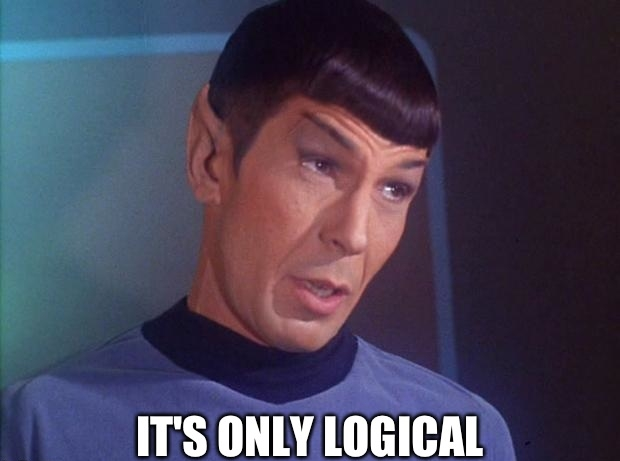
\includegraphics[height=0.8\textheight]{spock.jpg}
\end{frame}

\begin{frame}{Let's Express This Problem in Logic!}
  \begin{itemize}
  \item Let \structure{$M$} and \structure{$N$} be sets (i.e., \alert{domains}) such that \structure{$|M| = m$}, and \structure{$|N| = n$}
  \item Let \structure{$P \subseteq M \times N$} be a relation (i.e., \alert{predicate}) over sets \structure{$M$} and \structure{$N$}
  \item We can describe all of the constraints in first-order logic
    \begin{itemize}
    \item \pause each attendee gets a seat (i.e., at least one seat)
      \[
      \forall x \in M. \exists y \in N. P(x, y)
      \]
    \item \pause one person cannot occupy multiple seats
      \[
      \forall x \in M. \forall y, z \in N. P(x, y) \land P(x, z) \Rightarrow y=z
      \]
    \item \pause one seat cannot accommodate multiple attendees
      \[
      \forall w, x \in M. \forall y \in N. P(w, y) \land P(x, y) \Rightarrow w=x
      \]
    \end{itemize}
  \end{itemize}
  \pause
  The first two sentences constrain \structure{$P$} to be a function, and the last one makes it injective.
  \onslide<6>{
    \begin{tikzpicture}[remember picture,overlay]
      \node at (current page.center) {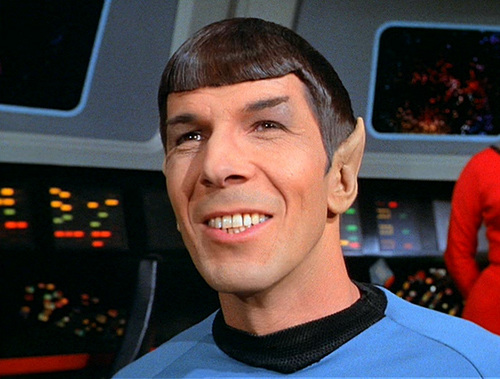
\includegraphics[height=0.4\textheight]{happy.jpg}};
    \end{tikzpicture}
  }
\end{frame}
% one could also add probabilities to these sentences to say that, e.g., there is a 1% probability of somebody taking up two seats, somebody sitting on somebody else's lap, somebody sitting on the floor, etc.

\begin{frame}{Overview of the Problem}
  \begin{itemize}
  \item \alert{First-order model counting} is the problem of counting the models of a sentence in first-order logic.
  \item The \alert{(symmetric) weighted} variation of the problem adds weights (e.g., probabilities) to predicates.
  \item Thus, SWFOMC can also be used for efficient \alert{probabilistic inference} in relational models.
  \item None of the (implemented) (SW)FOMC algorithms are able to count, e.g., \alert{injective} and \alert{bijective} functions.
  \end{itemize}
\end{frame}

% TODO: this can be fixed via recursion. Add a numerical example, show its complexity.
\begin{frame}{Recursion to the Rescue!}
  \[
  f(m, n) =
  \begin{cases}
    1 & \text{if } m = 0 \text{ and } n = 0 \\
    0 & \text{if } m > 0 \text{ and } n = 0 \\
    f(m, n-1) + mf(m-1, n-1) & \text{otherwise.}
  \end{cases}
  \]
  \begin{itemize}
  \item Optimal time complexity to compute \structure{$n^{\underline{m}}$} is \structure{$\Theta(\log m)$}
  \end{itemize}
\end{frame}

\end{document}
